\documentclass[12pt]{article}

\usepackage[utf8]{inputenc}
\usepackage[T1]{fontenc}
\usepackage{lmodern}
\usepackage[spanish]{babel}
\usepackage{booktabs}
\usepackage{amsmath}
\usepackage{forest}
\usepackage{float}
\usepackage{listings}
\usepackage{xcolor}
\usepackage{tikz}
\usepackage{enumitem}

\definecolor{codegreen}{rgb}{0,0.6,0}
\definecolor{codegray}{rgb}{0.5,0.5,0.5}
\definecolor{codepurple}{rgb}{0.58,0,0.82}
\definecolor{backcolour}{rgb}{0.95,0.95,0.92}

\lstdefinestyle{mystyle}{
    backgroundcolor=\color{backcolour},   
    commentstyle=\color{codegreen},
    keywordstyle=\color{magenta},
    numberstyle=\tiny\color{codegray},
    stringstyle=\color{codepurple},
    basicstyle=\ttfamily\footnotesize,
    breakatwhitespace=false,         
    breaklines=true,                 
    captionpos=b,                    
    keepspaces=true,                 
    numbers=left,                    
    numbersep=5pt,                  
    showspaces=false,                
    showstringspaces=false,
    showtabs=false,                  
    tabsize=2
}

\lstset{style=mystyle}

\sloppy
\setlength{\parindent}{0pt}

\begin{document}

% Título y materia
\begin{center}
  {\LARGE \textbf{Parcialito 2}}\\[0.5em]
  {Investigación Operativa, Universidad de San Andrés}
\end{center}

Los puntos 1 y 2 corresponden al tema A, mientras que los puntos 3 y 4 corresponden al tema B. Si encuentran algún error en el documento o hay alguna duda, mandenmé un mail a rodriguezf@udesa.edu.ar y lo revisamos.

\section{Cadenas de Markov - Esferas Pintadas}

\subsection{Enunciado}
Considere una caja que contiene actualmente dos esferas duras (tipo bolas de billar) sin pintar. Elegimos una esfera al azar y tiramos una moneda. Si la moneda sale cara, pintamos la esfera de rojo y si es seca la pintamos de negro. Si la esfera ya fue pintada entonces, independientemente del resultado de la moneda, cambiamos su color (de rojo a negro o de negro a rojo).

\begin{itemize}
    \item[a)] (3 pt.) Determine todos los posibles estados del sistema, considerando un vector [U, R, N] que representa cantidad de esferas sin pintar (unpainted), rojas o negras.
    \item[b)] (3 pt.) Determine la matriz de transición del problema y obtenga un grafo que la represente.
    \item[c)] (1.5 pt.) Suponga que parte del estado [0,0,2]. Calcule las probabilidades de:
    \begin{itemize}
        \item Tras dos esferas extraídas, tener el estado [0,2,0]
        \item Tras una esfera extraída, tener el estado [0,1,1]
    \end{itemize}
    \item[d)] (2.5 pt.) Plantee un sistema de ecuaciones que permita encontrar las probabilidades estacionarias del problema. ¿Qué representan en este contexto?
\end{itemize}

\subsection{Resolución}

\subsubsection{a) Estados Posibles}

Los estados posibles son vectores [U, R, N] donde:
\begin{itemize}
    \item U: número de esferas sin pintar (0, 1 o 2)
    \item R: número de esferas rojas (0, 1 o 2)
    \item N: número de esferas negras (0, 1 o 2)
\end{itemize}

Con la restricción de que U + R + N = 2 (total de esferas), los estados posibles son:
\begin{itemize}
    \item [2,0,0]: Estado inicial, dos esferas sin pintar
    \item [1,1,0]: Una sin pintar, una roja
    \item [1,0,1]: Una sin pintar, una negra
    \item [0,2,0]: Dos esferas rojas
    \item [0,0,2]: Dos esferas negras
    \item [0,1,1]: Una roja, una negra
\end{itemize}

\subsubsection{b) Matriz de Transición y Grafo}

La matriz de transición P, donde las filas y columnas representan los estados [0,1,1], [0,2,0], [0,0,2], [2,0,0], [1,1,0], [1,0,1] en ese orden, es:

\[
P = \begin{pmatrix}
0 & \frac{1}{2} & \frac{1}{2} & 0 & 0 & 0 \\
1 & 0 & 0 & 0 & 0 & 0 \\
1 & 0 & 0 & 0 & 0 & 0 \\
0 & 0 & 0 & 0 & \frac{1}{2} & \frac{1}{2} \\
\frac{1}{4} & \frac{1}{4} & 0 & 0 & 0 & \frac{1}{2} \\
\frac{1}{4} & 0 & \frac{1}{4} & 0 & \frac{1}{2} & 0
\end{pmatrix}
\]

Las probabilidades de 1/4 aparecen cuando tenemos una esfera sin pintar y una pintada. En este caso:
\begin{itemize}
    \item La probabilidad de elegir la esfera sin pintar es 1/2
    \item La probabilidad de que la moneda salga cara o seca es 1/2
    \item Por lo tanto, la probabilidad conjunta es 1/2 * 1/2 = 1/4
\end{itemize}

Representemos el sistema con un grafo:

\begin{center}
    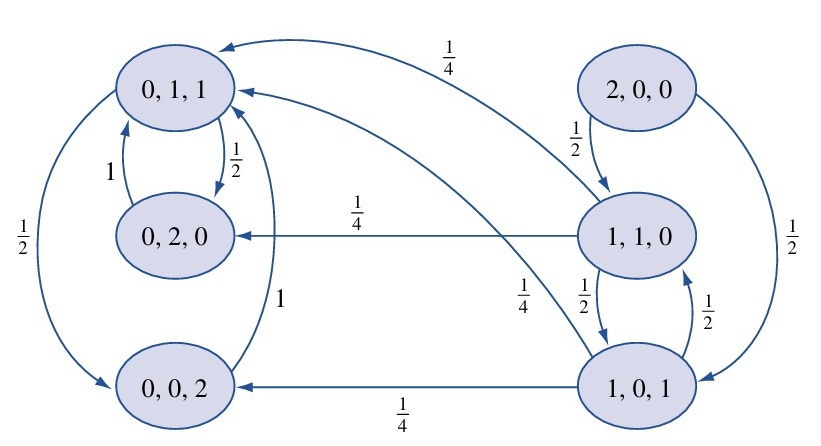
\includegraphics[width=0.8\textwidth]{img/grafo_esferas.jpeg}
\end{center}

\subsubsection{c) Probabilidades desde Estado [0,0,2]}

Partiendo del estado [0,0,2], necesitamos calcular:
\begin{itemize}
    \item La probabilidad de llegar al estado [0,2,0] después de dos extracciones
    \item La probabilidad de llegar al estado [0,1,1] después de una extracción
\end{itemize}

Paso 1: Probabilidad después de una extracción
\begin{itemize}
    \item Miramos la matriz P en la fila correspondiente al estado [0,0,2]
    \item La probabilidad de ir a [0,1,1] es 1
    \item Por lo tanto: P([0,1,1] | [0,0,2], 1 extracción) = 1
\end{itemize}

Paso 2: Probabilidad después de dos extracciones
\begin{itemize}
    \item Calculamos $P^2$ multiplicando P por sí misma:
    \[
    P^2 = \begin{pmatrix}
    \frac{1}{2} & \frac{1}{4} & \frac{1}{4} & 0 & 0 & 0 \\
    0 & \frac{1}{2} & \frac{1}{2} & 0 & 0 & 0 \\
    0 & \frac{1}{2} & \frac{1}{2} & 0 & 0 & 0 \\
    \frac{1}{8} & \frac{1}{8} & 0 & 0 & \frac{1}{4} & \frac{1}{2} \\
    \frac{3}{8} & \frac{1}{8} & \frac{1}{8} & 0 & \frac{1}{4} & \frac{1}{4} \\
    \frac{1}{8} & \frac{3}{8} & \frac{1}{8} & 0 & \frac{1}{4} & \frac{1}{4}
    \end{pmatrix}
    \]
    \item El estado [0,0,2] corresponde a la fila 3 de la matriz
    \item El estado [0,2,0] corresponde a la columna 2 de la matriz  
    \item Por lo tanto: $P^2_{3,2} = \frac{1}{2}$
    \item P([0,2,0] | [0,0,2], 2 extracciones) = 1/2
\end{itemize}

Paso 3: Resumen de resultados
\begin{itemize}
    \item Después de una extracción: 100\% de probabilidad de estar en [0,1,1]
    \item Después de dos extracciones: 50\% de probabilidad de estar en [0,2,0]
\end{itemize}

\subsubsection{d) Probabilidades Estacionarias}

Las probabilidades estacionarias $\pi$ son aquellas que satisfacen:
\[
\pi P = \pi \quad \text{y} \quad \sum_{i=1}^6 \pi_i = 1
\]

1) Primero escribimos la ecuación matricial usando la matriz P del problema:
\[
\begin{pmatrix} \pi_1 & \pi_2 & \pi_3 & \pi_4 & \pi_5 & \pi_6 \end{pmatrix} 
\begin{pmatrix}
0 & \frac{1}{2} & \frac{1}{2} & 0 & 0 & 0 \\
1 & 0 & 0 & 0 & 0 & 0 \\
1 & 0 & 0 & 0 & 0 & 0 \\
0 & 0 & 0 & 0 & \frac{1}{2} & \frac{1}{2} \\
\frac{1}{4} & \frac{1}{4} & 0 & 0 & 0 & \frac{1}{2} \\
\frac{1}{4} & 0 & \frac{1}{4} & 0 & \frac{1}{2} & 0
\end{pmatrix} = 
\begin{pmatrix} \pi_1 & \pi_2 & \pi_3 & \pi_4 & \pi_5 & \pi_6 \end{pmatrix}
\]

donde $\pi_1$ corresponde al estado [0,1,1], $\pi_2$ a [0,2,0], $\pi_3$ a [0,0,2], $\pi_4$ a [2,0,0], $\pi_5$ a [1,1,0] y $\pi_6$ a [1,0,1].

2) Realizando la multiplicación matriz-vector e igualando componente a componente:
\[
\begin{cases}
\frac{1}{4}\pi_5 + \frac{1}{4}\pi_6 = \pi_1 \\
\frac{1}{2}\pi_1 + \frac{1}{4}\pi_5 = \pi_2 \\
\frac{1}{2}\pi_1 + \frac{1}{4}\pi_6 = \pi_3 \\
0 = \pi_4 \\
\frac{1}{2}\pi_4 + \frac{1}{2}\pi_6 = \pi_5 \\
\frac{1}{2}\pi_4 + \frac{1}{2}\pi_5 = \pi_6 \\
\pi_1 + \pi_2 + \pi_3 + \pi_4 + \pi_5 + \pi_6 = 1
\end{cases}
\]

3) De la cuarta ecuación sabemos que $\pi_4 = 0$ (el estado [2,0,0] no puede ser alcanzado una vez que se pinta alguna esfera).

4) Resolviendo el sistema de ecuaciones:
\[
\pi = \begin{pmatrix} \frac{1}{3} & \frac{1}{6} & \frac{1}{6} & 0 & \frac{1}{6} & \frac{1}{6} \end{pmatrix}
\]

Interpretación:
\begin{itemize}
    \item A largo plazo, el estado [0,1,1] ocurre 1/3 del tiempo
    \item Los estados [0,2,0], [0,0,2], [1,1,0] y [1,0,1] ocurren cada uno 1/6 del tiempo
    \item El estado [2,0,0] nunca ocurre a largo plazo, ya que una vez que se pinta una esfera, nunca se puede volver a tener dos esferas sin pintar
\end{itemize}

Esta distribución es independiente de la distribución inicial y representa el equilibrio a largo plazo del sistema.

\section{Teoría de Inventarios - Muebles de Cocina}

\subsection{Enunciado}
Se tiene un local de redistribución de muebles de cocina. Se espera que este año la demanda llegue a 1200 unidades, distribuida de manera constante durante el año. El proveedor toma los pedidos con una plataforma online, lo que se traduce en un costo de \$400 por orden. El almacenamiento de muebles cuesta \$15 por unidad por mes.

\begin{itemize}
    \item[a)] (1 pt.) Si no se permiten faltantes, calcular la cantidad óptima para llenar el inventario y cada cuánto se hacen los pedidos. Suponga que no hay tiempo de espera entre orden y llegada.
    \item[b)] (1.5 pt.) Considere ahora que pasan 2 días entre pedido y llegada. Calcule el nivel del inventario para hacer el pedido sin incurrir en faltantes.
    \item[c)] (2 pt.) Si el costo extra es de \$500 por unidad no vendida, determine el nivel máximo de faltantes permitidos según el modelo EOQ.
    \item[d)] (2 pt.) Suponga que a partir del mes 10 la demanda aumenta un 25\% y aumenta el costo de orden a \$450. En las condiciones de (c), calcule los valores óptimos para los últimos dos meses del año.
    \item[e)] (3.5 pt.) Se quiere simular el costo anual total del modelo de inventario, pensando que la demanda es una variable aleatoria con distribución normal y que el costo de inventario sea una variable aleatoria con distribución uniforme. Observando el siguiente código, ¿es una simulación Montecarlo para este problema? Si no, ¿qué modificaría para que lo sea?
\begin{lstlisting}[language=Python]
# Parametros
D_prom = 1200  # demanda promedio anual
K = 400        # costo de orden
h_prom = 120   # costo de mantener promedio anual
L = 2          # tiempo de espera en dias
n_sim = 10000  # numero de simulaciones

# Generar muestras aleatorias
D_sims = np.random.normal(loc=D_prom, scale=0.1*D_prom, size=n_sim)
h_sims = np.random.uniform(low=0.8*h_prom, high=1.2*h_prom, size=n_sim)

# Asegurar valores positivos
D_sims = np.clip(D_sims, 1, None)
h_sims = np.clip(h_sims, 1e-3, None)

# Inicializar arrays para resultados
Q_sims = np.zeros(n_sim)
CT_sims = np.zeros(n_sim)
R_sims = np.zeros(n_sim)

# Simulacion Montecarlo
for i in range(n_sim):
    D_i = D_sims[i]
    h_i = h_sims[i]
    Q_i = np.sqrt((2*D_i*K)/h_i)
    CT_i = (D_i/Q_i)*K + (Q_i/2)*h_i
    R_i = D_i*(L/365)
    Q_sims[i] = Q_i
    CT_sims[i] = CT_i
    R_sims[i] = R_i
\end{lstlisting}
\end{itemize}

\subsection{Resolución}

\subsubsection{a) Cantidad Óptima sin Faltantes}

Para el modelo EOQ básico sin faltantes:

Datos:
\begin{itemize}
    \item D = 1200 unidades/año (demanda anual)
    \item K = \$400/orden (costo de ordenar)
    \item h = \$15/unidad-mes = \$180/unidad-año (costo de mantener)
\end{itemize}

La cantidad óptima a pedir (Q*) se calcula como:
\[
Q^* = \sqrt{\frac{2KD}{h}} = \sqrt{\frac{2 \cdot 400 \cdot 1200}{180}} = 47.14 \approx 47 \text{ unidades}
\]

El tiempo entre pedidos (T*) es:
\[
T^* = \frac{Q^*}{D} \cdot 12 = \frac{47}{1200} \cdot 12 = 0.47 \text{ meses} \approx 14 \text{ días}
\]

\subsubsection{b) Punto de Reorden}

La demanda diaria es:
\[
d = \frac{1200}{365} = 3.29 \text{ unidades/día}
\]

El punto de reorden (R) con lead time L = 2 días es:
\[
R = d \cdot L = 3.29 \cdot 2 = 6.58 \approx 7 \text{ unidades}
\]

El comportamiento del inventario será:
\begin{itemize}
    \item Cuando el nivel de inventario llega a 7 unidades, se realiza un pedido
    \item Durante los 2 días de lead time, se consumen aproximadamente 7 unidades
    \item El nuevo pedido llega justo cuando el inventario se acerca a 0
    \item El nivel de inventario sube a Q* = 47 unidades
\end{itemize}

\subsubsection{c) Modelo con Faltantes Permitidos}

Datos adicionales:
\begin{itemize}
    \item p = \$500/unidad (costo de faltante)
\end{itemize}

La cantidad óptima a pedir con faltantes ($Q_b^*$) es:
\[
Q_b^* = Q^* \sqrt{\frac{p}{p+h}} = 47 \sqrt{\frac{500}{500+180}} = 42.2 \approx 42 \text{ unidades}
\]

El nivel máximo de inventario ($S^*$) es:
\[
S^* = Q_b^* \cdot \frac{p}{p+h} = 42 \cdot \frac{500}{680} = 31.47 \approx 31 \text{ unidades}
\]

La cantidad máxima de faltantes ($B^*$) es:
\[
B^* = Q_b^* - S^* = 42 - 31 = 11 \text{ unidades}
\]

\subsubsection{d) Cambios en la Demanda y Costos para Faltantes}

Para los primeros 9 meses (usando el modelo con faltantes del punto c):
\begin{itemize}
    \item D = 1200 unidades/año
    \item K = \$400/orden
    \item h = \$180/unidad-año
    \item p = \$500/unidad (costo de faltante)
\end{itemize}

\[
Q_1^* = \sqrt{\frac{2KD}{h}} \sqrt{\frac{p}{p+h}} = 47 \cdot \sqrt{\frac{500}{680}} = 40.25 \approx 40 \text{ unidades}
\]

Para los últimos 3 meses (desde el mes 10):
\begin{itemize}
    \item D = 1500 unidades/año (25\% más)
    \item K = \$450/orden
    \item h = \$180/unidad-año
    \item p = \$500/unidad (costo de faltante)
\end{itemize}

\[
Q_2^* = \sqrt{\frac{2 \cdot 450 \cdot 1500}{180}} \sqrt{\frac{500}{680}} = 61.24 \cdot 0.857 = 52.5 \approx 53 \text{ unidades}
\]

El nivel máximo de inventario ($S^*$) para el período final:
\[
S^* = Q_2^* \cdot \frac{p}{p+h} = 53 \cdot \frac{500}{680} = 39 \text{ unidades}
\]

La cantidad máxima de faltantes ($B^*$) para el período final:
\[
B^* = Q_2^* - S^* = 53 - 39 = 14 \text{ unidades}
\]

\subsubsection{e) Simulación Monte Carlo}

Para realizar una simulación Monte Carlo, proponemos el siguiente código:

\begin{lstlisting}[language=Python]
import numpy as np

def simular_inventario(n_simulaciones):
    resultados = []
    for _ in range(n_simulaciones):
        # Generar demanda aleatoria (normal)
        D = np.random.normal(1200, 120)  # mu=1200, sigma=120
        
        # Generar costo inventario (uniforme)
        h = np.random.uniform(150, 190)  # entre $150 y $190
        
        # Generar costo faltante (uniforme)
        p = np.random.uniform(450, 550)  # entre $450 y $550
        
        # Calcular Q optimo con faltantes
        K = 400  # costo fijo
        Q = np.sqrt(2 * K * D / h) * np.sqrt(p / (p + h))
        
        # Calcular S optimo
        S = Q * (p / (p + h))
        
        # Calcular B optimo
        B = Q - S
        
        # Calcular costo total anual
        CT = K * D/Q + h * (S**2)/(2*Q) + p * (B**2)/(2*Q)
        
        resultados.append({
            'demanda': D,
            'costo_inventario': h,
            'costo_faltante': p,
            'Q_optimo': Q,
            'S_optimo': S,
            'B_optimo': B,
            'costo_total': CT
        })
    
    return resultados

# Ejecutar simulacion
resultados = simular_inventario(1000)

# Analizar resultados
# - Calcular estadisticas descriptivas
# - Generar histogramas
# - Identificar valores optimos mas frecuentes
\end{lstlisting}

Este código:
\begin{itemize}
    \item Genera valores aleatorios para la demanda usando distribución normal
    \item Genera valores aleatorios para el costo de inventario usando distribución uniforme
    \item Genera valores aleatorios para el costo de faltante usando distribución uniforme
    \item Calcula Q*, S*, B* y el costo total para cada simulación
    \item Permite analizar la distribución de los resultados
\end{itemize}

\section{Cadenas de Markov - Cargas de Trabajo}

\subsection{Enunciado}
Se necesita eficientizar el modelo de personal de una compañía y a tal fin se analizan las cargas de trabajo de los distintos grupos dentro de la empresa. Basado en las estadísticas de los últimos 6 meses, existen tres tipos de cargas de trabajo: ligera, media y pesada. El comportamiento mensual se ha caracterizado en términos de la probabilidad de que cambie su carga de trabajo de un mes a otro. Se ha obtenido que un grupo con carga ligera tiene un 15\% de probabilidades de pasar a tener carga media y un 4\% de pasar a tener carga pesada. Para los de carga media, tienen un 4\% para tener carga pesada y 6\% de carga ligera y para los de carga pesada, un 6\% de tener carga media y un 4\% de tener carga ligera.

\begin{itemize}
    \item[a)] (4.5 pt.) Describa el problema con un grafo y a partir del mismo escriba la matriz de transición de un problema de Markov.
    \item[b)] (1 pt.) ¿Cuál es la probabilidad de que un grupo con carga ligera tenga carga pesada en 2 meses?
    \item[c)] (2 pt.) La carga actual de un grupo depende de cuáles de sus tareas se confirman mes a mes. Actualmente, un grupo de trabajo tiene 65\% de probabilidades de tener carga pesada, 25\% de tener carga media y el resto de carga ligera. ¿Cómo se espera que sea la distribución de carga para el próximo mes?
    \item[d)] (2.5 pt.) Plantee un sistema de ecuaciones que permita encontrar las probabilidades estacionarias del sistema. ¿Qué representan en el contexto de este problema?
\end{itemize}

\subsection{Resolución}

\subsubsection{a) Grafo y Matriz de Transición}

Primero, calculemos las probabilidades de permanencia:
\begin{itemize}
    \item Carga ligera: 1 - 0.15 - 0.04 = 0.81
    \item Carga media: 1 - 0.06 - 0.04 = 0.90
    \item Carga pesada: 1 - 0.06 - 0.04 = 0.90
\end{itemize}

La matriz de transición P (Ligera, Media, Pesada) es:
\[
P = \begin{pmatrix}
0.81 & 0.15 & 0.04 \\
0.06 & 0.90 & 0.04 \\
0.04 & 0.06 & 0.90
\end{pmatrix}
\]

\shorthandoff{>}
\begin{center}
    \begin{tikzpicture}[node distance=3cm]
        \node[circle,draw] (L) {Ligera};
        \node[circle,draw] (M) [right of=L] {Media};
        \node[circle,draw] (P) [below of=L] {Pesada};
        
        \draw[->,bend left=20] (L) to node[above] {0.15} (M);
        \draw[->,bend left=20] (M) to node[above] {0.06} (L);
        \draw[->,bend left=20] (L) to node[left] {0.04} (P);
        \draw[->,bend left=20] (P) to node[left] {0.04} (L);
        \draw[->,bend left=20] (M) to node[right] {0.04} (P);
        \draw[->,bend left=20] (P) to node[right] {0.06} (M);
        
        \draw[->] (L) edge[loop above] node {0.81} ();
        \draw[->] (M) edge[loop above] node {0.90} ();
        \draw[->] (P) edge[loop below] node {0.90} ();
    \end{tikzpicture}
\end{center}
\shorthandon{>}

\subsubsection{b) Probabilidad de Carga Pesada en 2 Meses}

Calculamos $P^2$:
\[
P^2 = \begin{pmatrix}
0.81 & 0.15 & 0.04 \\
0.06 & 0.90 & 0.04 \\
0.04 & 0.06 & 0.90
\end{pmatrix}^2 = \begin{pmatrix}
0.6687 & 0.2589 & 0.0744 \\
0.1042 & 0.8214 & 0.0744 \\
0.0720 & 0.1140 & 0.8152
\end{pmatrix}
\]

Por lo tanto, $P^2_{1,3} = 0.0744$, lo que significa que la probabilidad de que un grupo con carga ligera tenga carga pesada en 2 meses es 7.44\%.

\subsubsection{c) Distribución Actual y Próxima}

Distribución actual: 10% ligera, 25% media, 65% pesada:
\[
\pi_0 = \begin{pmatrix} 0.10 & 0.25 & 0.65 \end{pmatrix}
\]

Distribución para el próximo mes:
\[
\pi_1 = \pi_0 P = \begin{pmatrix} 0.10 & 0.25 & 0.65 \end{pmatrix} \begin{pmatrix}
0.81 & 0.15 & 0.04 \\
0.06 & 0.90 & 0.04 \\
0.04 & 0.06 & 0.90
\end{pmatrix}
\]

Para obtener $\pi_1$ multiplicamos cada elemento de $\pi_0$ por su correspondiente columna en P y sumamos:

\begin{itemize}
    \item Primera componente: $0.10 \cdot 0.81 + 0.25 \cdot 0.06 + 0.65 \cdot 0.04 = 0.122$
    \item Segunda componente: $0.10 \cdot 0.15 + 0.25 \cdot 0.90 + 0.65 \cdot 0.06 = 0.264$
    \item Tercera componente: $0.10 \cdot 0.04 + 0.25 \cdot 0.04 + 0.65 \cdot 0.90 = 0.614$
\end{itemize}

\[
\pi_1 = \begin{pmatrix} 0.122 & 0.264 & 0.614 \end{pmatrix}
\]

Por lo tanto, en el próximo mes:
\begin{itemize}
    \item 12.2\% tendrán carga ligera
    \item 26.4\% tendrán carga media  
    \item 61.4\% tendrán carga pesada
\end{itemize}

\subsubsection{d) Probabilidades Estacionarias}

El sistema de ecuaciones es:
\[
\begin{cases}
0.81\pi_1 + 0.06\pi_2 + 0.04\pi_3 = \pi_1 \\
0.15\pi_1 + 0.90\pi_2 + 0.06\pi_3 = \pi_2 \\
0.04\pi_1 + 0.04\pi_2 + 0.90\pi_3 = \pi_3 \\
\pi_1 + \pi_2 + \pi_3 = 1
\end{cases}
\]

Resolviendo este sistema:
\[
\pi = \begin{pmatrix} 0.261 & 0.652 & 0.087 \end{pmatrix}
\]

Interpretación a largo plazo:
\begin{itemize}
    \item 26.1\% de los grupos tendrán carga ligera
    \item 65.2\% de los grupos tendrán carga media
    \item 8.7\% de los grupos tendrán carga pesada
\end{itemize}

Esta distribución es independiente de la distribución inicial y representa el equilibrio a largo plazo del sistema.

\section{Teoría de Colas - Banco}

\subsection{Enunciado}
Un banco recibe en promedio 12 clientes por hora y cada cajero atiende a razón de 18 clientes por hora. En principio, el banco puede contratar s cajeros que trabajan en filas en simultáneo y suponga que todas las filas que se forman delante de ellos son idénticas. El costo de espera es de \$10 por cliente-hora en cola y el costo de servicio es de \$15 por cajero-hora.

\begin{itemize}
    \item[a)] (0.5 pt.) Escriba el problema en notación de Kendall, explicando la elección de cada elemento.
    \item[b)] (1 pt.) Halle el factor de utilización y la capacidad ociosa como función de la cantidad de servidores s en el sistema.
    \item[c)] (2.5 pt.) Como las filas son idénticas, podemos analizar cada una por separado como sistemas de un solo servidor con capacidad infinita. Al llegar, los clientes eligen una de 4 filas de forma equiprobable. En estas condiciones, halle el largo promedio de la fila de espera frente al cajero y el tiempo que se pasa en ella.
    \item[d)] (2.5 pt.) Suponga que ahora cada fila puede tener un máximo de 3 clientes. Reobtenga lo que calculó en c) para este caso.
    \item[e)] (3.5 pt.) Observando el siguiente código, determine si el mismo es correcto para la simulación de este problema de filas. ¿Corresponde a una simulación Montecarlo? En caso de que no, ¿qué le agregaría para que lo sea?

\begin{lstlisting}[language=Python]
# Parametros
tasa_llegada   = 1    # lambda (llegadas/hora)
rate_atencion  = 15   # mu     (servicios por servidor por hora)
s              = 2    # numero de servidores
n_pasos        = 100  # numero de intervalos
costo_espera   = 10   # costo por cliente en cola
costo_servidor = 15   # costo por servidor

# Historial
hist_cola      = []
hist_atendidos = []

# Estado inicial
cola = 0

for paso in range(n_pasos):
    # 1) Llegadas:
    llegadas = np.random.normal(rate_llegada)
    cola += llegadas
    # 2) Atenciones
    capacidad = np.random.poisson(s * rate_atencion)
    atendidos = min(cola, capacidad)
    cola -= atendidos
    # 3) Guardar historial
    hist_cola.append(cola)
    hist_atendidos.append(atendidos)

# 4) Costo final
cola_final = hist_cola[-1]
costo_total = costo_espera * cola_final + costo_servidor * s
\end{lstlisting}
\end{itemize}

\subsection{Resolución}

\subsubsection{a) Notación de Kendall}

El sistema se puede describir como M/M/s/$\infty$/$\infty$/FIFO donde:
\begin{itemize}
    \item \textbf{M} (llegadas): El proceso de llegadas es Markoviano (Poisson) con $\lambda$ = 12 clientes/hora
    \item \textbf{M} (servicio): El tiempo de servicio es exponencial con $\mu$ = 18 clientes/hora por servidor
    \item \textbf{s}: Numero de servidores en paralelo (variable a optimizar)
    \item \textbf{$\infty$}: Capacidad del sistema (infinita)
    \item \textbf{$\infty$}: Tamano de la poblacion (infinita)
    \item \textbf{FIFO}: Disciplina de la cola (First In First Out)
\end{itemize}

\subsubsection{b) Capacidad Productiva y Ociosa}

Para un sistema M/M/s:
\begin{itemize}
    \item Tasa de llegadas: $\lambda$ = 12 clientes/hora
    \item Tasa de servicio por servidor: $\mu$ = 18 clientes/hora
    \item Intensidad de tráfico: $\rho$ = $\lambda$/(s$\mu$) = 12/(18s) = 2/3s
\end{itemize}

Para que el sistema sea estable necesitamos $\rho$ < 1, por lo tanto:
\[
\frac{2}{3s} < 1 \implies s > \frac{2}{3}
\]

La capacidad productiva es $\rho$ = 2/3s y la capacidad ociosa es 1 - $\rho$ = 1 - 2/3s.

\subsubsection{c) Tiempo en Cola y Largo con Un Servidor}

Para cada fila individual:
\begin{itemize}
    \item Tasa de llegadas por fila: $\lambda_{fila}$ = $\lambda$/4 = 3 clientes/hora
    \item Tasa de servicio: $\mu$ = 18 clientes/hora
    \item Intensidad de tráfico: $\rho_{fila}$ = $\lambda_{fila}$/$\mu$ = 3/18 = 1/6
\end{itemize}

Para un sistema M/M/1, las fórmulas son:
\[
L_q = \frac{\rho^2}{1-\rho} = \frac{(1/6)^2}{1-1/6} = \frac{1/36}{5/6} = \frac{1}{30} \text{ clientes}
\]

\[
W_q = \frac{L_q}{\lambda_{fila}} = \frac{1/30}{3} = \frac{1}{90} \text{ horas} = 40 \text{ segundos}
\]

\subsubsection{d) Sistema con Cola Limitada}

Para un sistema M/M/1/K con K = 4 (1 servidor + 3 en cola):
\begin{itemize}
    \item $\lambda_{fila}$ = 3 clientes/hora
    \item $\mu$ = 18 clientes/hora
    \item $\rho$ = 1/6
    \item K = 4
\end{itemize}

Las fórmulas para este caso son:
\[
P_0 = \frac{1-\rho}{1-\rho^{K+1}} = \frac{1-1/6}{1-(1/6)^5} = \frac{5/6}{1-1/7776} \approx 0.833
\]

\[
L_q = \frac{\rho^2(1-\rho^K)}{(1-\rho)(1-\rho^{K+1})} - \rho = \frac{(1/6)^2(1-(1/6)^3)}{(1-1/6)(1-(1/6)^4)} - \frac{1}{6} \approx 0.033 \text{ clientes}
\]

\[
W_q = \frac{L_q}{\lambda_{fila}(1-P_K)} = \frac{0.033}{3(1-0.833)} \approx 0.059 \text{ horas} \approx 3.5 \text{ minutos}
\]

\subsubsection{e) Análisis del Código}

El código proporcionado intenta simular un sistema de colas, pero tiene varios problemas y no constituye una simulación Monte Carlo adecuada:

\begin{enumerate}
    \item \textbf{Problemas en los parámetros}:
    \begin{itemize}
        \item La tasa de llegada está configurada como 1 cliente/hora cuando debería ser 12
        \item La tasa de atención está en 15 cuando debería ser 18 clientes/hora
        \item No se considera que hay 4 filas independientes
    \end{itemize}

    \item \textbf{Problemas en el modelado}:
    \begin{itemize}
        \item Usa distribución normal para las llegadas cuando debería ser Poisson (proceso Markoviano)
        \item No considera el tiempo entre eventos sino intervalos fijos
        \item No maneja correctamente las 4 filas independientes
        \item No implementa el límite de 3 clientes por fila
    \end{itemize}

    \item \textbf{Problemas en el cálculo de costos}:
    \begin{itemize}
        \item Solo considera el costo de la cola final, no el promedio durante toda la simulación
        \item No considera el tiempo que cada cliente pasa en la cola
    \end{itemize}
\end{enumerate}

Para convertirlo en una simulación Monte Carlo apropiada, se deberían hacer las siguientes modificaciones:

\begin{lstlisting}[language=Python]
import numpy as np
from numpy.random import exponential, poisson

def simular_banco(n_simulaciones, tiempo_simulacion):
    resultados = []
    
    # Parametros correctos
    lambda_total = 12    # llegadas por hora
    mu = 18             # atenciones por hora por servidor
    n_filas = 4         # numero de filas
    lambda_fila = lambda_total/n_filas  # llegadas por fila
    max_cola = 3        # maximo de clientes en cola
    
    for _ in range(n_simulaciones):
        # Inicializar filas
        colas = [[] for _ in range(n_filas)]
        tiempos_espera = []
        tiempo_actual = 0
        
        while tiempo_actual < tiempo_simulacion:
            # Generar proxima llegada (tiempo entre llegadas exponencial)
            t_llegada = exponential(1/lambda_total)
            tiempo_actual += t_llegada
            
            # Elegir fila aleatoriamente
            fila = np.random.randint(n_filas)
            
            # Si hay espacio en la fila
            if len(colas[fila]) < max_cola:
                # Generar tiempo de servicio
                t_servicio = exponential(1/mu)
                colas[fila].append(t_servicio)
                tiempos_espera.append(sum(colas[fila]))
            
            # Procesar servicios completados
            for i in range(n_filas):
                if colas[i]:
                    colas[i][0] -= t_llegada
                    while colas[i] and colas[i][0] <= 0:
                        colas[i].pop(0)
        
        # Calcular metricas
        L_q = np.mean([len(cola) for cola in colas])
        W_q = np.mean(tiempos_espera)
        costo = (costo_espera * L_q + costo_servidor * n_filas)
        
        resultados.append({
            'L_q': L_q,
            'W_q': W_q,
            'costo_total': costo
        })
    
    return resultados

# Ejecutar simulacion
resultados = simular_banco(1000, 24)  # 1000 simulaciones de 24 horas
\end{lstlisting}

Las mejoras principales incluyen:
\begin{itemize}
    \item Uso de distribuciones correctas (exponencial para tiempos entre llegadas y servicios)
    \item Manejo de múltiples filas independientes
    \item Implementación del límite de clientes por fila
    \item Seguimiento de tiempos de espera individuales
    \item Cálculo correcto de métricas promedio ($L_q$ y $W_q$)
    \item Múltiples simulaciones para obtener distribuciones de resultados
\end{itemize}

Esta versión sí constituye una simulación Monte Carlo apropiada ya que:
\begin{itemize}
    \item Utiliza generación de números aleatorios para modelar la incertidumbre
    \item Realiza múltiples iteraciones independientes
    \item Permite obtener distribuciones de las métricas de interés
    \item Modela correctamente la naturaleza estocástica del sistema
\end{itemize}

\end{document} 